% \documentclass{WHUBachelor}% 选项 forprint: 交付打印时添加, 避免彩色链接字迹打印偏淡. 即使用下一行:
 \documentclass[forprint]{WHUBachelor}
  \lstset{ 
    basicstyle=\small,% 
    escapeinside=``,% 
    keywordstyle=\color{red} \bfseries,% \underbar,% 
    identifierstyle={},% 
    commentstyle=\color{blue},% 
    stringstyle=\ttfamily,% 
    %labelstyle=\tiny,% 
    breaklines=true,
    extendedchars=false,% 
    linewidth=\textwidth,% 
    numbers=left,% 
    numberstyle=\tiny \color{blue},% 
    frame=trbl% 
    }


\begin{document}
%%%%%%% 下面的内容, 据实填空.

\title{实验项目四:中断机制的建立,用户程序与内核的解耦,以及用户程序的时间片轮转}
\Cschoolname{数据科学与计算机学院}          % 学院名
\Cmajor{计算机科学与技术}                  % 专业中文名
\StudentNumber{16337237} % 填写自己的学号
\author{王永锋}                            % 作者名字
\Csupervisor{凌应标}        %指导教师中文名、职称
\date{二〇一八年四月十七日}                % 日期, 要注意和英文日期一致!!

%----------------------------------------------------------------------------
\pdfbookmark[0]{封面}{title}         % 封面页加到 pdf 书签
\maketitle
\frontmatter
\pagenumbering{Roman}              % 正文之前的页码用大写罗马字母编号.
%-----------------------------------------------------------------------------
% \include{includefile/frontmatter}    % 加入摘要, 申明.
%==========================把目录加入到书签==============================%%%%%%
\pdfbookmark[0]{目录}{toc}
\tableofcontents
\mainmatter %% 以下是正文

%%%%%%%%%%%%%%%%%%%%%%%%%%%%%%%%%%%%%%%%%%%%%%%%%%%%%%%%%%%%%%%%%%%%%%%%%%%%%%%%%%%%%
%【实验方案】包括:硬件或虚拟机配置方法、软件工具与作用、方案的思想、相关原理、程序流程、算法和数据结构、程序关键模块,结合代码与程序中的位置位置进行解释。不得抄袭,否则按作弊处理。
%【实验过程】包括:主要工具安装使用过程及截图结果、程序过程中的操作步骤、测试数据、输入及输出说明、遇到的问题及解决情况、关键功能或操作的截图结果。不得抄袭,否则按作弊处理。
%【实验总结】每人必需写一段,文字不少于500字,可以写心得体会、问题讨论与思考、新的设想、感言总结或提出建议等等。不得抄袭,否则按作弊处理。
%【参考文献】(如有要列出,包括网上资源)
%%%%%%%%%%%%%%%%%%%%%%%%%%%--------main matter-------%%%%%%%%%%%%%%%%%%%%%%%%%%%%%%%%%%%%
\chapter{实验目的及要求}

\section{实验目的}

\begin{enumerate}
  \item 操作系统中断机制的建立,并学会如何使用中断实现系统调用。
  \item 使用C程序编写用户程序,并通过编写C运行时库,让用户程序与系统内核解耦合
  \item 尝试通过修改时钟中断,实现用户进程的时间片轮转运行。
\end{enumerate}

\section{实验要求}

本次实验,要求需要完成以下目标:\\

\begin{itemize}
  \item 实验四必须在实验三基础上进行,保留或扩展原有功能,实现部分新增功能。
  \item 内核中,对33号、34号、35号和36号中断编写中断服务程序,分别在屏幕1/4区域内显示一些个性化信息。
  \item 再编写一个用户程序,利用int 33、int 34、int 35和int 36产生中断调用你这4个服务程序。
  \item 扩充系统调用,实现三项以上新的功能,并编写一个测试所有系统调用功能的用户程序。
  \item 编写键盘中断响应程序,原有的你设计的用户程序运行时,键盘事件会做出有事反应:当键盘有按键时,屏幕适当位置显示”OUCH! OUCH!”。
  \item 制作包含引导程序,监控程序和若干可加载并执行的用户程序组成的1.44M软盘映像。
  \item 在指定时间内,提交所有相关源程序文件和软盘映像文件,操作使用说明和实验报告。
  \item 实验报告格式不变,实验方案丶实验过程或心得体会中主要描述个人工作,必须有展示技术性的过程细节截图和说明。
\end{itemize}

\chapter{实验方案}

\section{实验工具和环境}

本次实验环境与之前变化不大,唯一的改变是因为需要生成静态链接库,使用了linux系统中提供的ar工具。以下是本次实验的工具链。\autoref{tab:tools}

\begin{table}[htp]
  \caption{本实验所使用的工具链}
  \centering
  \begin{tabular}{cc}
    \toprule
    软件名称 & 用途  \\
    \midrule
    bash & 一个命令行终端,可提供linux的一些命令与执行shell脚本 \\
    nasm & 将x86汇编文件编译成.bin二进制文件 \\
    gcc & 编译工具,将c编译成二进制文件 \\
    ar & 使用多个.o 文件,生成.a静态链接库  \\
    ld & gcc套件中包含的连接器,用于将多个可执行文件连接起来 \\
    make & gcc套件中的工具,用于执行makefile文件 \\
    dd & 将二进制文件的内容写进软盘镜像中  \\
    objdump & 对可执行文件或二进制文件进行反编译 \\
    hexdump & 以十六进制形式查看软盘镜像文件 \\
    bochs & 虚拟机,用于加载装有自定义引导程序的软盘,使用软件模拟,速度不稳定  \\
    bochsdbg & 调试工具,用于给装有自定义引导程序的软盘文件进行调试 \\
    qemu & 虚拟机,用于加载装有自定义程序的软盘,使用硬件模拟,速度稳定且较快 \\
    \bottomrule
  \end{tabular}
  \label{tab:tools}
\end{table}

\section{程序功能说明及大致思路阐述}

这里会对程序的大致运行流程进行一个粗略的描述,同时罗列了当前系统内核支持的功能。

\subsection{程序大致思路阐述}

\begin{enumerate}
  \item 一开机,处于软盘第一个扇区的引导程序加载位于第40-45个扇区的加载器到内存0x8000处,并跳转到加载器中。
  \item 加载器(loader)使用文件系统的接口,加载位于第40-86个扇区的系统内核到内存0x10000处,并将控制权转交给系统内核。
  \item 系统内核刚开始运行,先进行初始化工作,(如初始化自定义中断,初始化文件系统数据,初始化进程控制块表)
  \item 调用文件系统接口,将指定文件加载到指定内存地址处
  \item 安装8号时钟中断,并且调用restart函数开始第一个进程。
\end{enumerate}

\subsection{实验四主要工作说明}

在上一个实验中,我已经实现了终端,自定义中断以及时钟中断的修改,同时还实现了文件系统。在这一次实验中,我主要做了以下工作:

\begin{itemize}
  \item 因为操作系统内核越来越大,18个扇区远远不够用,因此在引导扇区与内核之间增加了加载器,加载器能够使用文件系统的接口,读取内核所在扇区,如此便可摆脱18个扇区的限制。
  \item 将用户C库中最底层的四个函数包装成软中断,从而实现与操作系统解耦合。
  \item 在保证用户C库不依赖操作系统的数据后,整理C库文件,使用ar生成静态链接库,从而能够直接通过链接C库的方式直接生成用户程序,而不需要让用户程序与内核一起编译。
  \item 保证用户程序能够正常编译运行后,考虑到要让用户程序与内核的段分开(原来是在一个段上的),因此考虑使用进程切换的方式,实现切换段运行用户程序。
  \item 设计编写了进程控制块,并使用进程控制块与自定义时钟中断,实现多个用户程序的并发执行。
\end{itemize}

\subsection{实验结果不足,未来展望}

本次实验还有很多想完成的,碍于时间问题,先完成这一部分,下面是我觉得这一次做的不够好的地方,这也是之后我工作的方向。

\begin{itemize}
  \item 原先写的tty.c命令行终端,是依附于内核的,它必须使用内核才能够访问的全局变量,这导致了我无法将用户程序的并发执行与终端的运行放到一起。因此在这一次实验结果的镜像中,并没有看到上一次实验的终端。
  \item C库与内核的解耦合。操作系统的很多服务,我都需要使用中断的方式,包装成系统调用,从而能够让C库中通过调用中断,避免了与内核数据的直接交互,以此,实现与操作系统的解耦合。本次实验我将一部分函数从内核中使用中断抽象出接口,从而实现了解耦合,但是还有一些操作系统服务没能包含在用户C库中(如文件系统相关操作),这也是我没能将终端从内核中分离出来的主要原因。下一步,就是要继续完善系统调用,构建功能更加丰富的用户C库。
  \item 在创建进程的时候我是采用手动分配内存的方式,这样并不优美的做法,让我萌生了编写内存分配的想法,有了内存分配就可以进一步编写创建进程映像的系统调用,这样子我的操作系统就更加完满了。
\end{itemize}

\section{代码框架的设计}

\subsection{用户静态库的设计}

为了能够在C中更有效的操作硬件,同时保证更有效率的开发,我实现了以下库函数作为内核需要调用的头文件。对于一些无法使用C语言实现的功能,如端口的读写,我使用汇编语言实现了一些函数,将端口读写封装成一个个C语言直接可用的函数,而对bios中断的使用也是类似,在basic.asm中实现了对一些bios中断的直接调用,那么在C中,就可以对这些硬件操作进行进一步的封装(主要在stdio.c中实现),实现一些对开发者友好的接口,从而加快开发操作系统的效率。

以下是我用户C库的文件组织。

\begin{lstlisting}[language={[x86masm]Assembler}]
├── lib
│   ├── basic.asm
│   ├── makefile
│   ├── stdio.c
│   ├── string.c
│   └── style.c
\end{lstlisting}

\begin{table}[htp]
  \caption{库文件说明}
  \centering
  \rowcolors{1}{White}{Lavender}
  \begin{tabular}{lp{11cm}}
    \toprule
    头文件名 & 功能说明 \\
    \midrule
    basic.asm & 实现一些只能通过汇编实现的接口函数 \\
    stdio.c & 存放处理I/O的函数(如printf) \\
    string.c & 用于字符串的处理,包括比较strcmp和复制strcpy等函数 \\
    style.c & 编写了一个用于移动一行显示内容的函数,以后可以考虑做图形接口相关函数 \\
    \bottomrule
    \hiderowcolors
  \end{tabular}
  \label{tab:library}
\end{table}

\subsubsection{部分函数的函数调用图}

库中对用户的每一个接口,其底层都是依赖于系统内核已经编写好的33,34,35,36号中断及一些bios中断提供的功能。下面举两例:putc函数与printf函数。

\begin{figure}[htp]
  \centering
  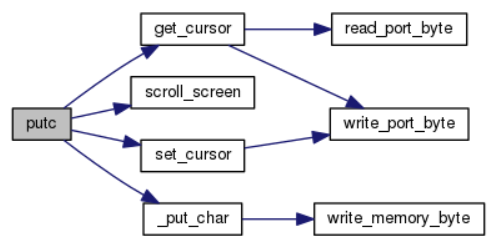
\includegraphics[width=13cm]{"./figure/putc-call-graph.png"}
  \caption{putc函数的函数调用图}
  \label{fig:putc}
\end{figure}

\begin{figure}[htp]
  \centering
  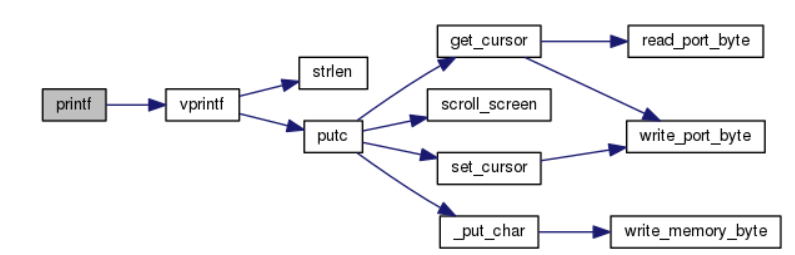
\includegraphics[width=13cm]{"./figure/printf-call-graph.png"}
  \caption{printf函数的函数调用图}
  \label{fig:printf}
\end{figure}

对于putc函数的执行,以下放出简短的源代码方便理解该函数如何与内核解耦合。
本函数没有直接调用biox的中断,而是通过端口交互的方式,修改光标,然后调用底层的_put_char()函数来将指定的字母写到显存中,这样做是为了以后可以不依赖bios中断,从而有可能能够尝试保护模式。

最底层的三个函数,read_port_byte(),write_port_byte, write_memory_byte,使用了中断的方式,调用了操作系统提供的功能,来对端口进行读写,以及进行写内存。这里要用中断实现写内存的考虑主要是想在内核中判断该地址是否合法,可能用户想写一些内核的关键区域,这时候是应该要阻止的。

\begin{lstlisting}[language=c]
void putc(char c){
    u16 cursor_index = get_cursor();
    u16 row = cursor_index / 80;
    u16 col = cursor_index % 80;
    if (cursor_index >= 1920){
        scroll_screen();
        cursor_index = 1840;
    }
    switch (c) {
        case '\n':
            set_cursor((row+1)*80); // 回车,移到下一行
            break;
        case '\r':
            set_cursor(row*80);    // 移到本行开头处
            break;
        default:
            _put_char(c, cursor_index);
            set_cursor(cursor_index+1);
            break;
    }
    return ;
}
\end{lstlisting}

\subsubsection{静态链接库}

在将C库与操作系统解耦合之后,我们可以讲C库连接成一个静态链接库,这样子多个用户程序都可以链接同一个C运行时库,不用重新编译。我是用的是下面的指令:

\begin{lstlisting}[language=c]
	ar rcs ../include/c_run_time.a stdio.o  basic.o  string.o  style.o
\end{lstlisting}

此后需要编译用户程序的时候,只需要这样写即可:

\begin{lstlisting}[language=c]
  ld $(LINK_FLAGS) -o test_a.bin test_a.o ../include/c_run_time.a
  // LINK_FLAGS = -Ttext 0x00000 -m elf_i386 -T t.lds --oformat binary
\end{lstlisting}


\subsection{进程控制块的设计}
TODO:


\subsection{自定义时钟中断,实现切换进程}
TODO:


\chapter{实验难点及亮点}
TODO:

\chapter{曾经遇到的问题}
TODO:

\chapter{实验结果}
TODO:

\section{进程切换的测试}
TODO:

\chapter{实验总结}

这是实验四的实验总结。

这一次实验四做的比较慢,主要是因为其实之前已经算是把ppt上的要求做好了,然后一开始也不知道自己要朝着怎样的目标去做,这时候又有其他课程的项目需要做,于是就把很多时间放在了其他课程的项目。

大概还是维持着初衷吧,想着要尽量将操作系统的实现超前一个星期,所以在这一次实验中,除去为整理文件结构,分离用户程序与系统内核所做的努力,我的时间主要花在了实现进程切换的功能上,可以说是花了整整两天时间从早到晚不停地打码调试进程切换。对编写时钟中断后的调试,甚至可以说花了我一天时间去观察时钟中断对栈的操作是否正确。有一段时间,三个用户程序切换个几百次后就会崩溃,就会跳转到一个非法地址,面对这种概率性出现的问题,我一开始几乎没有debug的思路,超绝望,怕自己完不成这一次实验。

后来吧,平静下来了,想看看栈的情况如何,经过细细的调试,看到我的用户程序每回来一次,用户栈就会往后退两个字节,看到这个现象的我,就像是看到了一点点黑暗中的曙光啊。至少到这时候是可以确定是我对栈的操作出了一点问题,后来重写了几遍时钟中断,调试了很多遍,终于发现,是自己用了一条"push sp"这样一条机器相关的指令,我对这条指令的理解与机器不一致,导致出现问题。

怎么说呢,在调试的过程,极其需要耐心,因为这需要我仔细的查看汇编,找到C代码对应的汇编代码的位置,然后在bochs上一步一步的走下去,查看寄存器的值,这一次的bug,也是我一步一步的看栈的值,才看到这样一个与自己心理预期不一致的情况,这才终于发现关键的问题所在,最终才解决这个问题。

说起来,操作系统编程中,其实有一个需求特别需要满足:能够使用gdb调试!因为我们自己编写的C代码,现阶段我们甚至没有办法通过C指令的单步调试来缩小问题范围,而只能通过更加底层的汇编来进行排查问题。而据我了解,qemu虚拟机是可以和gdb调试器联动,实现C源码级别的调试功能。我希望,下一次能够整理出一套C源码级调试的方案,不仅方便自己,也方便大家调试吧。

当然,多看点汇编也并无坏处,在这几次实验中,我不断重复地查看汇编代码,寻找其中部分与自己心理预期不一致的代码,也据此了解了不少gcc编译代码时会出现的行为,如结构体的自动对齐,函数调用帧栈的处理等等,同时还了解到gcc生成汇编时是默认四段合一,所有段寄存器都是相同的,这个坑到了不少人,我听说过一些同学由于有一个段寄存器和别的不同,C代码中刚好又生成了依赖这个段寄存器的代码,导致出现了极其难排查的bug。从这个角度上说,汇编级别的debug是必不可少的,不过有了C代码级别的调试,相必我们调试的速度会更上一层楼。


%%%============================================%%%

%%%=== 参考文献 ========%%%



% \cleardoublepage\phantomsection
% \addcontentsline{toc}{chapter}{参考文献}

\bibliography{opsystem}
% \bibliographystyle{unsrt}

% \begin{thebibliography}{00}
%   \bibitem{r1} 作者. 文章题目 [J].  期刊名, 出版年份,卷号(期数): 起止页码.
%   \bibitem{r2} 作者. 书名 [M]. 版次. 出版地:出版单位,出版年份:起止页码.
%   \bibitem{r3} 邓建松等, 《\LaTeXe~科技排版指南》, 科学出版社.
%   \bibitem{r4} 吴凌云, 《CTeX~FAQ (常见问题集)》, \textit{Version~0.4}, June 21, 2004.
%   \bibitem{r5} Herbert Vo\ss, Mathmode, \url{http://www.tex.ac.uk/ctan/info/math/voss/mathmode/Mathmode.pdf}.


% \end{thebibliography}

% \include{includefile/backmatter} %%%致谢

%%%-------------- 附录. 不需要可以删除.-----------
\appendix

\chapter{文件的组织}
\label{code:organization}
\begin{lstlisting}[language={[x86masm]Assembler}]
  .
  ├── a.img
  ├── bochsrc.bxrc
  ├── boot
  │   ├── boot.asm
  │   ├── fat.asm
  │   ├── loader.c
  │   ├── loader.lds
  │   ├── loader_start.asm
  │   ├── loader_start.h
  │   ├── makefile
  │   └── root.asm
  ├── include
  │   ├── basic.h
  │   ├── c_run_time.a
  │   ├── fsystem.h
  │   ├── global.h
  │   ├── kernel_run_time.a
  │   ├── macro.inc
  │   ├── proc.h
  │   ├── stdio.h
  │   ├── string.h
  │   ├── style.h
  │   ├── system_call.h
  │   ├── type.h
  │   └── utilities.h
  ├── kernel
  │   ├── kernel.asm
  │   ├── makefile
  │   ├── start.c
  │   └── t.lds
  ├── lib
  │   ├── basic.asm
  │   ├── makefile
  │   ├── stdio.c
  │   ├── string.c
  │   └── style.c
  ├── service
  │   ├── fsystem.c
  │   ├── global.c
  │   ├── makefile
  │   ├── proc.c
  │   ├── system_call.c
  │   └── tty.c
  ├── makefile
  ├── readme.md
  └── user
      ├── makefile
      ├── ouch.c
      ├── test_a.c
      ├── test_b.c
      └── t.lds
\end{lstlisting}

\chapter{int 8h 的实现}

\label{code:int_8h}
\begin{lstlisting}[language={[x86masm]Assembler}] 
TODO:
\end{lstlisting}


\cleardoublepage
\end{document}